\documentclass[12pt,a4paper]{book}

\usepackage[top=3cm,right=3.5cm,bottom=3cm,left=3cm]{geometry}
\renewcommand{\baselinestretch}{1.7}
\usepackage{amssymb}
\usepackage[fleqn]{amsmath}

\usepackage{xcolor}

\usepackage{tikz,pgfplots}
\pgfplotsset{compat=1.12}
\usepgfplotslibrary{fillbetween}
\usetikzlibrary{patterns}
\usetikzlibrary{positioning}
\usetikzlibrary{arrows,automata}

\begin{document}
Page $365$\\\\\\
The actual non-left recursive grammar is 
\begin{align*}
&A \to Ba/b\\
&B \to bdB′/eB′/bdB″/eB″\\
&B′ \to cB′\in\\
&B″ \to adB″/\in
\end{align*}
26. Construct the equivalent fi nite automata from the following regular grammar.
\begin{align*}
&S \to aS/bA/b\\
&A \to aA/bS/a
\end{align*}
\textbf{Solution:} In the grammar, there are two non-terminals S and A. So, in the fi nite automata, there
are three states. For the production S $\to$ aS, the transitional diagram is
For the production S $\to$ bA, the transitional diagram is
\begin{center}
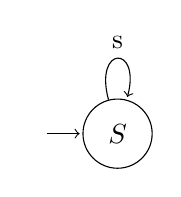
\begin{tikzpicture}[shorten >=1pt,node distance=5cm,on grid,auto]
   \node[initial,state,initial text=] (s) {$S$}; 
   \draw[->] (s) edge [loop above] node  {s} (s);
 \end{tikzpicture}
 \end{center}
 For the production S $\to$ bA, the transitional diagram is
\begin{center}
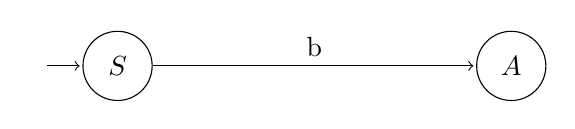
\begin{tikzpicture}[shorten >=1pt,node distance=5cm,on grid,auto]
   \node[initial,state,initial text=] (s) {$S$}; 
   \node[state](a) [right=of s] {$A$};
   \draw[->] (s) edge node  {b} (a);
 \end{tikzpicture}
 \end{center}
For the production S $\to$ b, the transitional diagram is
\begin{center}
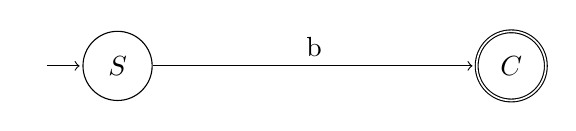
\begin{tikzpicture}[shorten >=1pt,node distance=5cm,on grid,auto]
   \node[initial,state,initial text=] (s) {$S$}; 
   \node[state,accepting](a) [right=of s] {$C$};
   \draw[->] (s) edge node  {b} (a);
 \end{tikzpicture}
 \end{center}
For the ‘S’ production, the complete transitional diagram is
\begin{center}
\begin{tikzpicture}[shorten >=1pt,node distance=5cm,on grid,auto]
   \node[initial,state,initial text=] (s) {$S$}; 
   \node[state,accepting](c) [ below right=of s] {$C$};
   \draw[->] (s) edge [loop above] node  {a} (s);
   \node[state](a) [right=of s] {$A$};
   \draw[->] (s) edge node  {b} (a);
   \draw[->] (s) edge node  {b} (c);
 \end{tikzpicture}
 \end{center}
For the ‘A’ production, the transitional diagram is
\begin{center}
\begin{tikzpicture}[shorten >=1pt,node distance=5cm,on grid,auto]
   \node[initial,state,initial text=] (s) {$S$}; 
   \node[state,accepting](c) [ below right=of s] {$C$};
   \draw[->] (a) edge [loop above] node  {a} (a);
   \node[state](a) [right=of s] {$A$};
   \draw[->] (s) edge node  {b} (a);
   \draw[->] (a) edge node  {a} (c);
 \end{tikzpicture}
 \end{center}
The complete transitional diagram for the previous grammar is
\begin{center}
\begin{tikzpicture}[shorten >=1pt,node distance=5cm,on grid,auto]
   \node[initial,state,initial text=] (s) {$S$}; 
   \node[state,accepting](c) [ below right=of s] {$C$};
   \draw[->] (s) edge [loop above] node  {a} (s);
   \draw[->] (a) edge [loop above] node  {a} (a);
   \node[state](a) [right=of s] {$A$};
   \draw[->] (s) edge [bend left=10] node[above] {b} (a);
   \draw[->] (a) edge [bend left=10] node [below] {b} (s);
   \draw[->] (a) edge node  {a} (c);
   \draw[->] (s) edge node  {b} (c);
 \end{tikzpicture}
 \end{center}\newpage
 Page $366$\\\\\\
27. Construct the equivalent fi nite automata from the following regular grammar.
\begin{align*}
&S \to Aa\\
&A \to Sb/Ab/\in
\end{align*}
\textbf{Solution:} The grammar accepts null string. So, A is the fi nal state. For the production rule A $\to \in$ ,\\
the  transitional  diagram  is
\begin{center}
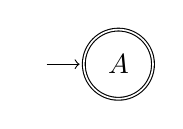
\begin{tikzpicture}[shorten >=1pt,node distance=5cm,on grid,auto]
   \node[initial,state,initial text=,accepting] (s) {$A$}; 
 \end{tikzpicture}
 \end{center}
For the production S $\to$ Aa, the  transitional  diagram is
\begin{center}
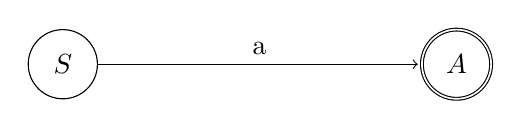
\begin{tikzpicture}[shorten >=1pt,node distance=5cm,on grid,auto]
   \node[state] (s) {$S$}; 
   \node[state,accepting](a) [right=of s] {$A$};
   \draw[->] (s) edge node  {a} (a);
 \end{tikzpicture}
 \end{center}
For the production A $\to$ Sb/Ab, the transitional diagram is
\begin{center}
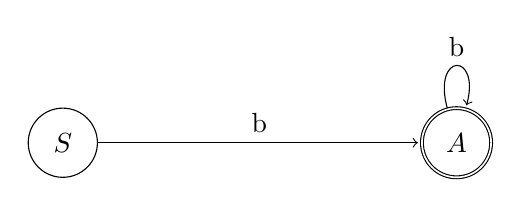
\begin{tikzpicture}[shorten >=1pt,node distance=5cm,on grid,auto]
   \node[state] (s) {$S$}; 
   \node[state,accepting](a) [right=of s] {$A$};
   \draw[->] (s) edge node  {b} (a);
   \draw[->] (a) edge [loop above] node  {b} (a);
 \end{tikzpicture}
 \end{center}
The complete transitional diagram is
\begin{center}
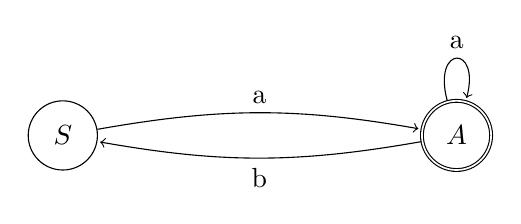
\begin{tikzpicture}[shorten >=1pt,node distance=5cm,on grid,auto]
   \node[state] (s) {$S$}; 
   \node[state,accepting](a) [right=of s] {$A$};
   \draw[->] (a) edge [loop above] node  {a} (b);
   \draw[->] (s) edge [bend left=10] node[above] {a} (a);
   \draw[->] (a) edge [bend left=10] node [below] {b} (s);
 \end{tikzpicture}
 \end{center}
28. Using this lemma, prove that  $L =\{a^i b^j | j = i2\}$ is not a CFL.$\quad \left[ WBUT 2009 (IT)\right]$\\
\textbf{Solution:}
Step I: Assume that the language set L is a CFL. Let n be a natural number obtained by using the
pumping lemma.\\
Step II: Let z = $aib2i. So, | z | = 3i . Let 3i > n$. According to the pumping lemma for CFL, we can
write z = uvwxy, where $| vx | \geq 1 and | vwx | \leq n$.\\
Step III: The string z contains ‘a’ and ‘b’, and so v and x will be in any of the following forms.\\
i) Contain only a, i.e., in the form $a^x$\\
ii) Contain only b, i.e., in the form $b^y$\\
iii) Contain the repetition of ‘a’ and ‘b’, i.e., in the form $a^xb^y$\\
For case (i), if we take k = 2, then $uv^2wx^2y$ cannot be in the form of $a^i b^j$ $|$ j = $i^2$,\\
For case (ii),if we take k = 2, then $uv^2wx^2y$cannot be in the form of $a^i b^j$ $|$ j = $i^2$,\\
For case (iii),if we take k=0, then $uv^2wx^2y$ cannot be in the form of $a^i b^j$ $|$ j = $i^2$,\\
For the three cases, we are getting a contradiction,and so $L={a^i b^j | j = i^2}$is not a CFL.\\
29. Verify whether the languages generated by the following grammar are fi nite or not. If fi nite, find
the longest string generated by the grammar.
\begin{align*}
a)&S \to Ab \quad\quad && b) S \to AB\\
&A \to aB/a \quad\quad   &&A \to CD\\
&B \to bS \quad\quad    &&B \to CD\\
& &&C \to aD\\
& &&D \to b
\end{align*}\newpage
 Page $367$\\\\\\
\textbf{Solution:} \\
a) The grammar is not in CNF. The grammar converted to CNF is
\begin{align*}
&S \to AC\\
&A \to AB/a\\
&B \to CS\\
&C \to b
\end{align*}
In the grammar, there are four non-terminals. For this reason, in the directed graph for the
grammar, there are four nodes. The directed graph is
\begin{center}
\begin{tikzpicture}[shorten >=1pt,node distance=5cm,on grid,auto]
   \node[state] (s) {$S$}; 
   \node[state](a) [below left=of s] {$A$};
   \node[state](c) [below right=of s] {$C$};
   \node[state](b) [below=of s] {$B$};
   \draw[->] (a) edge [loop left] node  {} (b);
   \draw[->] (s) edge node  {} (a);
   \draw[->] (s) edge node  {} (c);
   \draw[->] (a) edge node  {} (c);
   \draw[->] (a) edge node  {} (b);
   \draw[->] (b) edge node  {} (c);
   \draw[->] (b) edge node  {} (s);
 \end{tikzpicture}
 \end{center}
The graph contains loop. So, the language generated by the CFG is infi nite.\\
b) The grammar is not in CNF. To make the grammar in CNF, the productions are as follows
\begin{align*}
&S \to AB\\
&A \to CD\\
&B \to CD\\
&C \to ED\\
&D \to b\\
&E \to a
\end{align*}
In the grammar, there are six non-terminals. For this reason, in the directed graph for the
grammar, there are six nodes.\\
The directed graph for the grammar is
\begin{center}
\begin{tikzpicture}[shorten >=1pt,node distance=5cm,on grid,auto]
   \node[state] (s) {$S$}; 
   \node[state](a) [below left=of s] {$A$};
   \node[state](c) [below=of a] {$C$};
   \node[state](b) [below right=of s] {$B$};
   \node[state](d) [below=of b] {$D$};
   \node[state](e) [below left=of a] {$E$};
   \draw[->] (s) edge node  {} (a);
   \draw[->] (s) edge node  {} (b);
   \draw[->] (a) edge node  {} (c);
   \draw[->] (a) edge node  {} (d);
   \draw[->] (b) edge node  {} (c);
   \draw[->] (b) edge node  {} (d);
   \draw[->] (c) edge node  {} (d);
   \draw[->] (c) edge node  {} (e);
 \end{tikzpicture}
 \end{center}
The directed graph does not contain any loop. So, the grammar is fi nite. The length of the
string generated by the grammar is 6.\newpage
Page $368$\\\\\\
1. Context-free language is language.
\begin{align*}
&a) Type 0 \quad  &&b) Type 1\\
&c) Type 2 &&d) Type 3
\end{align*}
2. Parsing a string from a given grammar means
\begin{align*}
&a)\text{ Finding a derivation}\\
&b) \text{Finding a leftmost derivation}\\
&c)\text{ Finding a rightmost derivation}\\
&d)\text{ Finding a derivation tree.}
\end{align*}
3. A grammar is called ambiguous if
\begin{align*}
&a) \text{It generates more than one string}\\
&b)\text{ It generates both leftmost and rightmost derivation for a given string}\\
&c) \text{It generates more than one parse tree for a given string}\\
&d)\text{ It fulfi lls both (b) and (c)}
\end{align*}
4. Which is not true for ambiguous grammar?
\begin{align*}
&a) \text{Ambiguity creates problem in generating a language from a given grammar}\\
&b) \text{All ambiguity can be removed.}\\
&c) \text{Inherent ambiguity cannot be removed}\\
&d) \text{Some ambiguity can be removed by hand}
\end{align*}
5. Non-generating symbols are those symbols
which
\begin{align*}
&a) \text{Do not generate any string of nonterminals}\\
&b) \text{Do not generate any null string}\\
&c) \text{Do not generate any string of terminal and non-terminals}\\
&d) \text{Go not generate any string of terminals}
\end{align*}
6. Useless symbols in CFG are
\begin{align*}
&a) \text{Non-generating symbols and nonreachable symbols}\\
&b) \text{Null alphabets and null string}\\
&c) \text{Non-terminal symbols}\\
&d) \text{All of these}
\end{align*}
7. Which of the following is a unit production?
\begin{align*}
&a) \text{(String of NT)} \to \text{(String of NT)}\\
&b) \text{(Single NT)} \to \text{(String of NT)}\\
&c) \text{(Single NT)} \to \text{(Single NT)}\\
&d) \text{(String of NT)} \to \text{(Single NT)}
\end{align*}
8. Which is true for the following CFG?
\[S \to aA/\in \]
\[A \to bA/a \]
\begin{align*}
&a)\text{ Null production can be removed} \\
&b) \text{Null production cannot be removed} \\
&c) \text{As A does not produce null, null cannot be removed} \\
&d)\text{ Both (b) and (c)}
\end{align*}
9. Which of the following production is in CNF? (more specifi c)
\begin{align*}
&a) (NT) \to \text{(String of NT)}\\
&b) (NT) \to \text{(String of terminal and nonterminal)}\\
&c) (NT) \to \text{(String of terminal)}\\
&d) (NT) \to \text{(String of exactly two NT)}
\end{align*}
10. Which of the following production is in GNF? (more specifi c)
\begin{align*}
&a) (NT) \to \text{(Single T)(String of NT)}\\
&b) (NT) \to \text{(Single NT)(String of T)}\\
&c) (NT) \to \text{(String of terminal and nonterminal)}\\
&d) (NT) \to \text{(String of NT)}
\end{align*}
11. Which of the following is common in both CNF and GNF?
\begin{align*}
&a) (NT) \to \text{(Single T)(String of NT)}\\
&b) (NT) \to \text{(String of exactly two NT)}\\
&c) (NT) \to \text{(String of NT)}\\
&d) (NT) \to \text{(Single T)}
\end{align*}
12. Context-free language is not closed under
\begin{align*}
&a) \text{Union} \quad &&\text{b) Concatenation}\\
&c) \text{Complementation} &&\text{d) Star closure}
\end{align*}
Answers:
\begin{align*}
&1. c \quad 2. a\quad 3. c\quad 4. b \quad5. d \quad6. a\\
&7. c \quad8. b \quad9. d \quad10. a \quad11. d \quad 12. c
\end{align*}
\end{document}